\documentclass[12pt, titlepage]{article}
\usepackage{float}
\usepackage{booktabs}
\usepackage{tabularx}
\usepackage{hyperref}
\usepackage{graphicx}
\usepackage{float}
\usepackage{soul}
\usepackage{geometry}
\geometry{margin = 0.75in}
\hypersetup{
    colorlinks,
    citecolor=black,
    filecolor=black,
    linkcolor=black,
    urlcolor=blue
}
\usepackage[round]{natbib}

\title{SE 3XA3: Test Report\\Space Invader}

\author{L03,G07
		\\ Qianlin Chen and chenq84
		\\ Jiacheng Wu and wuj187
		\\ Tingyu Shi and shit19
}

\date{\today}



\begin{document}

\maketitle

\pagenumbering{roman}
\tableofcontents
\listoftables

\newpage
\begin{table}[htb]
\caption{\bf Revision History}
\begin{tabularx}{\textwidth}{p{3cm}p{2cm}X}
\toprule {\bf Date} & {\bf Version} & {\bf Notes}\\
\midrule
April 11 & All team members & Finish the document\\
\bottomrule
\end{tabularx}
\end{table}

\newpage

\pagenumbering{arabic}

\noindent This document specifies the complete testing process for Space Invader. It contains an evaluation of the project's functional and non-functional requirements that are defined in our SRS, the changes made due to testing result, and analysis of the traceability between requirements and modules.

\section{Functional Requirements Evaluation}

\subsection{Model}
\begin{table}[h!]
\scalebox{0.85}{
\begin{tabularx}{\textwidth}{p{3cm}X}
\toprule
\textbf{Test 1} & \textbf{Test-FR15-M1} \\\\
\textbf{Description} & Test if scores are added after bullets from aircraft hit monsters\\\\
\textbf{Type} & Unit test(functional, dynamic, automated)\\\\
\textbf{Initial State} & Bullet from aircraft hits one of the monsters.\\\\
\textbf{Input} & getScore() is called on Score object.\\\\
\textbf{Expected} & Player's score increase.\\\\
\textbf{Output} & Player's score increase.\\\\
\textbf{Result} & \textbf{PASS}\\

\bottomrule
\end{tabularx}
}
\end{table}
\begin{table}[h!]
\scalebox{0.85}{
\begin{tabularx}{\textwidth}{p{3cm}X}
\toprule
\textbf{Test 2} & \textbf{Test-FR16-M2} \\\\
\textbf{Description} & Test if life point decrements after aircraft get hit\\\\
\textbf{Type} & Unit test(functional, dynamic, automated)\\\\
\textbf{Initial State} & Monster's bullets hit aircraft\\\\
\textbf{Input} & getLives() is called on SpaceShip object\\\\
\textbf{Expected} & Aircraft's live decreases\\\\
\textbf{Output} & Aircraft's live decreases\\\\
\textbf{Result} & \textbf{PASS}\\

\bottomrule
\end{tabularx}
}
\end{table}
\begin{table}[h!]
\scalebox{0.85}{
\begin{tabularx}{\textwidth}{p{3cm}X}
\toprule
\textbf{Test 3} & \textbf{Test-FR16-M3} \\\\
\textbf{Description} & Test if life point increments after aircraft hits heart item\\\\
\textbf{Type} & Unit test(functional, dynamic, automated)\\\\
\textbf{Initial State} & Bullets from aircraft hit the health game item in the monster matrix\\\\
\textbf{Input} & getLives() is called on SpaceShip object\\\\
\textbf{Expected} & Aircraft's live increases by 1\\\\
\textbf{Output} & Aircraft's live increases by 1\\\\
\textbf{Result} & \textbf{PASS}\\

\bottomrule
\end{tabularx}
}
\end{table}
\begin{table}[h!]
\scalebox{0.85}{
\begin{tabularx}{\textwidth}{p{3cm}X}
\toprule
\textbf{Test 4} & \textbf{Test-FR25-M4} \\\\
\textbf{Description} & Test if isDead() return true after green monster get hit\\\\
\textbf{Type} & Unit test(functional, dynamic, automated)\\\\
\textbf{Initial State} & A green monster is hit by one bullet from the aircraft\\\\
\textbf{Input} & isDead() is called on Monster object\\\\
\textbf{Expected} & isDead() return true\\\\
\textbf{Output} & isDead() return true\\\\
\textbf{Result} & \textbf{PASS}\\

\bottomrule
\end{tabularx}
}
\end{table}
\begin{table}[h!]
\scalebox{0.85}{
\begin{tabularx}{\textwidth}{p{3cm}X}
\toprule
\textbf{Test 5} & \textbf{Test-FR26-M5} \\\\
\textbf{Description} & Test if isDead() return true after blue monster get hit twice\\\\
\textbf{Type} & Unit test(functional, dynamic, automated)\\\\
\textbf{Initial State} & A blue monster is hit by two bullets from the aircraft\\\\
\textbf{Input} & isDead() is called on Monster object\\\\
\textbf{Expected} & isDead() return true\\\\
\textbf{Output} & isDead() return true\\\\
\textbf{Result} & \textbf{PASS}\\

\bottomrule
\end{tabularx}
}
\end{table}
\begin{table}[h!]
\scalebox{0.85}{
\begin{tabularx}{\textwidth}{p{3cm}X}
\toprule
\textbf{Test 6} & \textbf{Test-FR27-M6} \\\\
\textbf{Description} & Test if isDead() return true after pink monster get hit three times\\\\
\textbf{Type} & Unit test(functional, dynamic, automated)\\\\
\textbf{Initial State} & A pink monster is hit by three bullets from the aircraft\\\\
\textbf{Input} & isDead() is called on Monster object\\\\
\textbf{Expected} & isDead() return true\\\\
\textbf{Output} & isDead() return true\\\\
\textbf{Result} & \textbf{PASS}\\

\bottomrule
\end{tabularx}
}
\end{table}
\begin{table}[h!]
\scalebox{0.85}{
\begin{tabularx}{\textwidth}{p{3cm}X}
\toprule
\textbf{Test 7} & \textbf{Test-FR29-M7} \\\\
\textbf{Description} & Test if area of obstacle decrease after it gets hit by bullet\\\\
\textbf{Type} & Unit test(functional, dynamic)\\\\
\textbf{Initial State} & One bullet hits an obstacle\\\\
\textbf{Input} & No input will be given in this test case\\\\
\textbf{Expected} & The area of obstacles should decrease by observation\\\\
\textbf{Output} & area of obstacles decrease in our observation\\\\
\textbf{Result} & \textbf{PASS}\\

\bottomrule
\end{tabularx}
}
\end{table}
\begin{table}[h!]
\scalebox{0.85}{
\begin{tabularx}{\textwidth}{p{3cm}X}
\toprule
\textbf{Test 8} & \textbf{Test-FR30-M8} \\\\
\textbf{Description} & Test if the game item GUI disappears only after aircraft hits it\\\\
\textbf{Type} & Unit test(functional, dynamic, manual)\\\\
\textbf{Initial State} & Game GUI presents one game item, one monster and one aircraft\\\\
\textbf{Input} & Monster shoots one bullet to the game item firstly and aircraft shoots one bullet to the game item secondly\\\\
\textbf{Expected} & Game item disappears only after aircraft hits it\\\\
\textbf{Output} & Game item disappears only after aircraft hits it\\\\
\textbf{Result} & \textbf{PASS}\\

\bottomrule
\end{tabularx}
}
\end{table}
\begin{table}[h!]
\scalebox{0.85}{
\begin{tabularx}{\textwidth}{p{3cm}X}
\toprule
\textbf{Test 9} & \textbf{Test-FR31-M9} \\\\
\textbf{Description} & Test if number of game items is less than 5 for each round\\\\
\textbf{Type} & Unit test(functional, dynamic, manual)\\\\
\textbf{Initial State} & Start a new round\\\\
\textbf{Input} & No input is given but testers need to record the number of game items\\\\
\textbf{Expected} & The number of game items of each round is less than 5\\\\
\textbf{Output} & The number of game items of each round is less than 5\\\\
\textbf{Result} & \textbf{PASS}\\

\bottomrule
\end{tabularx}
}
\end{table}
\begin{table}[h!]
\scalebox{0.85}{
\begin{tabularx}{\textwidth}{p{3cm}X}
\toprule
\textbf{Test 10} & \textbf{Test-FR32-M10} \\\\
\textbf{Description} & Test if 4 random monsters eliminated after the aircraft hits the bomb item\\\\
\textbf{Type} & Unit test(functional, dynamic, manual)\\\\
\textbf{Initial State} & GUI displays a monster matrix with a bomb game item in it\\\\
\textbf{Input} & Testers operate the aircraft and shoot a bullet from the aircraft to the bomb item\\\\
\textbf{Expected} & 4 monsters eliminated from the monster matrix\\\\
\textbf{Output} & 4 monsters eliminated from the monster matrix\\\\
\textbf{Result} & \textbf{PASS}\\

\bottomrule
\end{tabularx}
}
\end{table}
\begin{table}[h!]
\scalebox{0.85}{
\begin{tabularx}{\textwidth}{p{3cm}X}
\toprule
\textbf{Test 11} & \textbf{Test-FR33-M11} \\\\
\textbf{Description} & Test if number of bullets increment after the aircraft hits the ammo item\\\\
\textbf{Type} & Unit test(functional, dynamic, manual)\\\\
\textbf{Initial State} & GUI displays a monster matrix with a ammo game item in it\\\\
\textbf{Input} & Testers operate the aircraft and shoot a bullet from the aircraft to the ammo item\\\\
\textbf{Expected} & number of bullet from the aircraft increases by 1\\\\
\textbf{Output} & number of bullet from the aircraft increases by 1\\\\
\textbf{Result} & \textbf{PASS}\\

\bottomrule
\end{tabularx}
}
\end{table}
\begin{table}[h!]
\scalebox{0.85}{
\begin{tabularx}{\textwidth}{p{3cm}X}
\toprule
\textbf{Test 12} & \textbf{Test-FR34-M12} \\\\
\textbf{Description} & Test if number of life points increment after the aircraft hits the heart item\\\\
\textbf{Type} & Unit test(functional, dynamic, manual)\\\\
\textbf{Initial State} & GUI displays a monster matrix with a heart game item in it\\\\
\textbf{Input} & Testers operate the aircraft and shoot a bullet from the aircraft to the heart item\\\\
\textbf{Expected} & number of life point from the aircraft increases by 1\\\\
\textbf{Output} & number of life point from the aircraft increases by 1\\\\
\textbf{Result} & \textbf{PASS}\\

\bottomrule
\end{tabularx}
}
\end{table}
\begin{table}[h!]
\scalebox{0.85}{
\begin{tabularx}{\textwidth}{p{3cm}X}
\toprule
\textbf{Test 13} & \textbf{Test-FR35-M13} \\\\
\textbf{Description} & Test if game items occur randomly within monster matrix\\\\
\textbf{Type} & Unit test(functional, dynamic, manual)\\\\
\textbf{Initial State} & Several monster matricess are loaded\\\\
\textbf{Input} & No input will be given in this test case, but testers need to make a screenshot for each monster matrix\\\\
\textbf{Expected} & Game items occur randomly in different matrices\\\\
\textbf{Output} & Game items occur randomly in different matrices according to the matrices\\\\
\textbf{Result} & \textbf{PASS}\\

\bottomrule
\end{tabularx}
}
\end{table}
\begin{table}[h!]
\scalebox{0.85}{
\begin{tabularx}{\textwidth}{p{3cm}X}
\toprule
\textbf{Test 14} & \textbf{Test-FR40-M14} \\\\
\textbf{Description} & Test if the aircraft shoots bullets after pressing SPACE\\\\
\textbf{Type} & Unit test(functional, dynamic, manual)\\\\
\textbf{Initial State} & Set a new game\\\\
\textbf{Input} & Testers shoot bullets by press SPACE\\\\
\textbf{Expected} & Aircraft shoots a bullet\\\\
\textbf{Output} & Aircraft shoots a bullet\\\\
\textbf{Result} & \textbf{PASS}\\

\bottomrule
\end{tabularx}
}
\end{table}
\newpage
\clearpage
\subsection{View}
\begin{table}[h!]
\scalebox{0.85}{
\begin{tabularx}{\textwidth}{p{3cm}X}
\toprule
\textbf{Test 15} & \textbf{Test-FR1-V1} \\\\
\textbf{Description} & Test if the GUI switch to choosing game mode after pressing any key\\\\
\textbf{Type} & Functional, Dynamic, Manual\\\\
\textbf{Initial State} & Welcome message has been displayed\\\\
\textbf{Input} & Testers enter any key\\\\
\textbf{Expected} & The GUI display a message and let testers to choose the play mode\\\\
\textbf{Output} & The GUI display a message and let testers to choose the play mode\\\\
\textbf{Result} & \textbf{PASS}\\

\bottomrule
\end{tabularx}
}
\end{table}
\begin{table}[h!]
\scalebox{0.85}{
\begin{tabularx}{\textwidth}{p{3cm}X}
\toprule
\textbf{Test 16} & \textbf{Test-FR2-V2} \\\\
\textbf{Description} & Test if GUI display instructions about monster type normally after tester chose the mode\\\\
\textbf{Type} & Functional, Dynamic, Manual\\\\
\textbf{Initial State} & Game mode selection UI hass been displayed\\\\
\textbf{Input} & Testers enter S or D to choose the play mode\\\\
\textbf{Expected} & GUI display the game instructions about monster types\\\\
\textbf{Output} & GUI display the game instructions about monster types\\\\
\textbf{Result} & \textbf{PASS}\\

\bottomrule
\end{tabularx}
}
\end{table}
\begin{table}[h!]
\scalebox{0.85}{
\begin{tabularx}{\textwidth}{p{3cm}X}
\toprule
\textbf{Test 17} & \textbf{Test-FR3-V3} \\\\
\textbf{Description} & Test if GUI display playing instructions normally after tester chose the mode\\\\
\textbf{Type} & Functional, Dynamic, Manual\\\\
\textbf{Initial State} & Game mode selection UI hass been displayed\\\\
\textbf{Input} & Testers enter S or D to choose the play mode\\\\
\textbf{Expected} & GUI display the game playing instructions \\\\
\textbf{Output} & GUI display the game playing instructions\\\\
\textbf{Result} & \textbf{PASS}\\

\bottomrule
\end{tabularx}
}
\end{table}
\begin{table}[h!]
\scalebox{0.85}{
\begin{tabularx}{\textwidth}{p{3cm}X}
\toprule
\textbf{Test 18} & \textbf{Test-FR4-V4} \\\\
\textbf{Description} & Test if GUI display scores in game correctly after testers enter the game\\\\
\textbf{Type} & Functional, Dynamic, Manual\\\\
\textbf{Initial State} & Monsters and game instructions have been displayed\\\\
\textbf{Input} & Testers press ENTER key\\\\
\textbf{Expected} & The game should display total score at the left up corner and the intial score should be 0 \\\\
\textbf{Output} & The game should display total score at the left up corner and the intial score should be 0\\\\
\textbf{Result} & \textbf{PASS}\\

\bottomrule
\end{tabularx}
}
\end{table}
\begin{table}[h!]
\scalebox{0.85}{
\begin{tabularx}{\textwidth}{p{3cm}X}
\toprule
\textbf{Test 19} & \textbf{Test-FR5-V5} \\\\
\textbf{Description} & Test if GUI display health points in game correctly after testers enter the game\\\\
\textbf{Type} & Functional, Dynamic, Manual\\\\
\textbf{Initial State} & Monsters and game instructions have been displayed\\\\
\textbf{Input} & Testers press ENTER key\\\\
\textbf{Expected} & The game should display health points at the beginning of the game and the number of items should be 5 \\\\
\textbf{Output} & The game should display 5 health points\\\\
\textbf{Result} & \textbf{PASS}\\

\bottomrule
\end{tabularx}
}
\end{table}
\begin{table}[h!]
\scalebox{0.85}{
\begin{tabularx}{\textwidth}{p{3cm}X}
\toprule
\textbf{Test 20} & \textbf{Test-FR6-V6} \\\\
\textbf{Description} & Test if the background of the game is displayed\\\\
\textbf{Type} & Functional, Dynamic, Manual\\\\
\textbf{Initial State} & Monsters and game instructions have been displayed\\\\
\textbf{Input} & Testers press ENTER key\\\\
\textbf{Expected} & The game should display the background \\\\
\textbf{Output} & The game display the background we set\\\\
\textbf{Result} & \textbf{PASS}\\

\bottomrule
\end{tabularx}
}
\end{table}
\begin{table}[h!]
\scalebox{0.85}{
\begin{tabularx}{\textwidth}{p{3cm}X}
\toprule
\textbf{Test 21} & \textbf{Test-FR7-V7} \\\\
\textbf{Description} & Test if the monster matrix of the game is displayed\\\\
\textbf{Type} & Functional, Dynamic, Manual\\\\
\textbf{Initial State} & Monsters and game instructions have been displayed\\\\
\textbf{Input} & Testers press ENTER key\\\\
\textbf{Expected} & The game should display the monster matrix \\\\
\textbf{Output} & The game display the monster matrix\\\\
\textbf{Result} & \textbf{PASS}\\

\bottomrule
\end{tabularx}
}
\end{table}
\begin{table}[h!]
\scalebox{0.85}{
\begin{tabularx}{\textwidth}{p{3cm}X}
\toprule
\textbf{Test 22} & \textbf{Test-FR8-V8} \\\\
\textbf{Description} & Test if the game items are displayed randomly\\\\
\textbf{Type} & Functional, Dynamic, Manual\\\\
\textbf{Initial State} & Monsters and game instructions have been displayed\\\\
\textbf{Input} & Testers press ENTER key and make a screenshot\\\\
\textbf{Expected} & The game items are displayed randomly in the screenshots \\\\
\textbf{Output} & The game items are displayed randomly in the screenshots\\\\
\textbf{Result} & \textbf{PASS}\\

\bottomrule
\end{tabularx}
}
\end{table}
\begin{table}[h!]
\scalebox{0.85}{
\begin{tabularx}{\textwidth}{p{3cm}X}
\toprule
\textbf{Test 23} & \textbf{Test-FR9-V9} \\\\
\textbf{Description} & Test if the game display number of aircraft correctly\\\\
\textbf{Type} & Functional, Dynamic, Manual\\\\
\textbf{Initial State} & Monsters and game instructions have been displayed\\\\
\textbf{Input} & Testers press S key and start the game\\\\
\textbf{Expected} & Game GUI display a single aircraft \\\\
\textbf{Output} & Game GUI display a single aircraft\\\\
\textbf{Result} & \textbf{PASS}\\

\bottomrule
\end{tabularx}
}
\end{table}
\begin{table}[h!]
\scalebox{0.85}{
\begin{tabularx}{\textwidth}{p{3cm}X}
\toprule
\textbf{Test 24} & \textbf{Test-FR9-V10} \\\\
\textbf{Description} & Test if the game display number of aircraft correctly\\\\
\textbf{Type} & Functional, Dynamic, Manual\\\\
\textbf{Initial State} & Monsters and game instructions have been displayed\\\\
\textbf{Input} & Testers press D key and start the game\\\\
\textbf{Expected} & Game GUI display two aircrafts \\\\
\textbf{Output} & Game GUI display aircrafts\\\\
\textbf{Result} & \textbf{PASS}\\

\bottomrule
\end{tabularx}
}
\end{table}
\begin{table}[h!]
\scalebox{0.85}{
\begin{tabularx}{\textwidth}{p{3cm}X}
\toprule
\textbf{Test 25} & \textbf{Test-FR10-V11} \\\\
\textbf{Description} & Test if the game display obstacles correctly\\\\
\textbf{Type} & Functional, Dynamic, Manual\\\\
\textbf{Initial State} & Monsters and game instructions have been displayed\\\\
\textbf{Input} & Testers press ENTER key and start the game\\\\
\textbf{Expected} & Game GUI display four obstacles between aircraft and monsters \\\\
\textbf{Output} & Game GUI display four obstacles between aircraft and monsters\\\\
\textbf{Result} & \textbf{PASS}\\

\bottomrule
\end{tabularx}
}
\end{table}
\begin{table}[h!]
\scalebox{0.85}{
\begin{tabularx}{\textwidth}{p{3cm}X}
\toprule
\textbf{Test 26} & \textbf{Test-FR11-V12} \\\\
\textbf{Description} & Test if the game display scores after the game\\\\
\textbf{Type} & Functional, Dynamic, Manual\\\\
\textbf{Initial State} & Testers finish the game\\\\
\textbf{Input} & No input is given\\\\
\textbf{Expected} & Scores are displayed \\\\
\textbf{Output} & Scores are displayed\\\\
\textbf{Result} & \textbf{PASS}\\

\bottomrule
\end{tabularx}
}
\end{table}
\begin{table}[h!]
\scalebox{0.85}{
\begin{tabularx}{\textwidth}{p{3cm}X}
\toprule
\textbf{Test 27} & \textbf{Test-FR12-V13} \\\\
\textbf{Description} & Test if the game display WIN after testers pass round 5\\\\
\textbf{Type} & Functional, Dynamic, Manual\\\\
\textbf{Initial State} & Testers aree in game round 5\\\\
\textbf{Input} & Testers pass game round 5\\\\
\textbf{Expected} & Game GUI display winning massage \\\\
\textbf{Output} & Game GUI display "WIN!"\\\\
\textbf{Result} & \textbf{PASS}\\

\bottomrule
\end{tabularx}
}
\end{table}
\begin{table}[h!]
\scalebox{0.85}{
\begin{tabularx}{\textwidth}{p{3cm}X}
\toprule
\textbf{Test 28} & \textbf{Test-FR13-V14} \\\\
\textbf{Description} & Test if the game display fail message after testers lose\\\\
\textbf{Type} & Functional, Dynamic, Manual\\\\
\textbf{Initial State} & Testers are in any game round\\\\
\textbf{Input} & Testers' aircraft's hp goes to zero\\\\
\textbf{Expected} & Game GUI display fail massage \\\\
\textbf{Output} & Game GUI display "FAIL!"\\\\
\textbf{Result} & \textbf{PASS}\\

\bottomrule
\end{tabularx}
}
\end{table}
\begin{table}[h!]
\scalebox{0.85}{
\begin{tabularx}{\textwidth}{p{3cm}X}
\toprule
\textbf{Test 29} & \textbf{Test-FR28-V16} \\\\
\textbf{Description} & Test if display of green monster is off after one hit\\\\
\textbf{Type} & Functional, Dynamic, Manual\\\\
\textbf{Initial State} & Testers start a game\\\\
\textbf{Input} & Testers shoot the green monster once\\\\
\textbf{Expected} & Display of green monster disappear \\\\
\textbf{Output} & Display of green monster disappear\\\\
\textbf{Result} & \textbf{PASS}\\

\bottomrule
\end{tabularx}
}
\end{table}
\begin{table}[h!]
\scalebox{0.85}{
\begin{tabularx}{\textwidth}{p{3cm}X}
\toprule
\textbf{Test 30} & \textbf{Test-FR28-V17} \\\\
\textbf{Description} & Test if display of blue monster is off after two hits\\\\
\textbf{Type} & Functional, Dynamic, Manual\\\\
\textbf{Initial State} & Testers start a game\\\\
\textbf{Input} & Testers shoot the blue monster twice\\\\
\textbf{Expected} & Display of blue monster disappear \\\\
\textbf{Output} & Display of blue monster disappear\\\\
\textbf{Result} & \textbf{PASS}\\

\bottomrule
\end{tabularx}
}
\end{table}
\begin{table}[h!]
\scalebox{0.85}{
\begin{tabularx}{\textwidth}{p{3cm}X}
\toprule
\textbf{Test 31} & \textbf{Test-FR28-V18} \\\\
\textbf{Description} & Test if display of pink monster is off after three hits\\\\
\textbf{Type} & Functional, Dynamic, Manual\\\\
\textbf{Initial State} & Testers start a game\\\\
\textbf{Input} & Testers shoot the pink monster three times\\\\
\textbf{Expected} & Display of pink monster disappear \\\\
\textbf{Output} & Display of pink monster disappear\\\\
\textbf{Result} & \textbf{PASS}\\

\bottomrule
\end{tabularx}
}
\end{table}
\newpage
\clearpage
\subsection{Controller}
\begin{table}[h!]
\scalebox{0.85}{
\begin{tabularx}{\textwidth}{p{3cm}X}
\toprule
\textbf{Test 32} & \textbf{Test-FR18-C2} \\\\
\textbf{Description} & Test if the game contain 5 rounds as designed\\\\
\textbf{Type} & Functional, Dynamic, Manual\\\\
\textbf{Initial State} & Game instructions and introduction to monsters have been displayed\\\\
\textbf{Input} & Testers try to pass the whole game and count the number of game rounds\\\\
\textbf{Expected} & number of game rounds is 5 \\\\
\textbf{Output} & number of game rounds is 5\\\\
\textbf{Result} & \textbf{PASS}\\

\bottomrule
\end{tabularx}
}
\end{table}
\begin{table}[h!]
\scalebox{0.85}{
\begin{tabularx}{\textwidth}{p{3cm}X}
\toprule
\textbf{Test 33} & \textbf{Test-FR23-C7} \\\\
\textbf{Description} & Test if the movement of monster matrix is correct\\\\
\textbf{Type} & Functional, Dynamic, Manual\\\\
\textbf{Initial State} & Testers are playing in different game rounds\\\\
\textbf{Input} & No input\\\\
\textbf{Expected} & The movement of the monster matrix is east-south-west \\\\
\textbf{Output} & The movement of the monster matrix is east-south-west\\\\
\textbf{Result} & \textbf{PASS}\\

\bottomrule
\end{tabularx}
}
\end{table}
\begin{table}[h!]
\scalebox{0.85}{
\begin{tabularx}{\textwidth}{p{3cm}X}
\toprule
\textbf{Test 34} & \textbf{Test-FR24-C8} \\\\
\textbf{Description} & Test if monsters in matrix shoot randomly in different rounds\\\\
\textbf{Initial State} & Testers are in different game rounds\\\\
\textbf{Input} & No input\\\\
\textbf{Expected} & Monsters in matrix shoot randomly in different rounds \\\\
\textbf{Output} & Monsters in matrix shoot randomly in different rounds\\\\
\textbf{Result} & \textbf{PASS}\\

\bottomrule
\end{tabularx}
}
\end{table}
\begin{table}[h!]
\scalebox{0.85}{
\begin{tabularx}{\textwidth}{p{3cm}X}
\toprule
\textbf{Test 35} & \textbf{Test-FR24-C9} \\\\
\textbf{Description} & Test if users can enter the game successfully\\\\
\textbf{Initial State} & Game instructions and introduction to monsters have been displayed\\\\
\textbf{Input} & Testers press ENTER key\\\\
\textbf{Expected} & GUI shows the game \\\\
\textbf{Output} & GUI shows the game\\\\
\textbf{Result} & \textbf{PASS}\\

\bottomrule
\end{tabularx}
}
\end{table}
\begin{table}[h!]
\scalebox{0.85}{
\begin{tabularx}{\textwidth}{p{3cm}X}
\toprule
\textbf{Test 36} & \textbf{Test-FR37-C10} \\\\
\textbf{Description} & Test if users are able to exit the game\\\\
\textbf{Initial State} & Testers are in any game round\\\\
\textbf{Input} & Testers press cross icon\\\\
\textbf{Expected} & Game exited \\\\
\textbf{Output} & Game exited\\\\
\textbf{Result} & \textbf{PASS}\\

\bottomrule
\end{tabularx}
}
\end{table}
\begin{table}[h!]
\scalebox{0.85}{
\begin{tabularx}{\textwidth}{p{3cm}X}
\toprule
\textbf{Test 37} & \textbf{Test-FR38-C11} \\\\
\textbf{Description} & Test if aircraft can be moved properly\\\\
\textbf{Initial State} & Aircraft is in a stationary state with a certain position\\\\
\textbf{Input} & Testers press keyboard to move the aircraft\\\\
\textbf{Expected} & Aircraft move to a correct position \\\\
\textbf{Output} & Aircraft moves the a position which is calculated correctly\\\\
\textbf{Result} & \textbf{PASS}\\

\bottomrule
\end{tabularx}
}
\end{table}
\newpage
\clearpage
\section{Nonfunctional Requirements Evaluation}
\subsection{Look and Feel Testing}

\textbf{Test 38: }\\
Test-NFR1-LF1\\
Type: Dynamic, Automated, Functional\\
Initial State: Game started.\\
Input/Condition: Testers use external tool to measure
 the FPS.\\
Output/Result: FPS value should always be greater than
30.\\
How test will be performed: Testers can record the FPS
of the game every 10 seconds and measure FPS for 2
minutes. After that, testers can check if all the 
values recorded are greater than 30.\\
\textbf{Result: PASS}\\\\
\textbf{Test 39:}\\
Test-NFR2-LF2\\
Type: Dynamic, Manual, Functional\\
Initial State: Game started.\\
Input/Condition: Testers record players' thoughts about 
the game display.\\
Output/Result: Over 80\% of people can recognize 
game elements clearly.\\ 
How test will be performed: Testing team
can invite 10 people to play the game and
8 out of 10 random persons should recognize all the elements clearly.\\
\textbf{Result: PASS}\\\\
\textbf{Test: 40}\\
Test-NFR3-LF3\\
Type: functional, dynamic, manual\\
Initial State: Game started.\\
Input/Condition: No inputs will be given for this 
test case. Players will be asked about their thoughts
about the game minimalism.\\
Output/Result: Over 80\% of players think the game
follows the style of minimalism.\\
How test will be performed: Invite 10 random persons to
play the game and then record their thoughts about the
game minimalism.\\
\textbf{Result: PASS}\\\\
\textbf{Test 41:}\\
Test-NFR4-LF4\\
Type: functional, dynamic, manual\\
Initial State: Game started.\\
Input/Condition: No inputs will be given for this 
test case. Players will be asked about their thoughts
about the game mood.\\
Output/Result: Over 80\% of players think the game
mood is intense.\\
How test will be performed: Invite 10 random persons to
play the game and then record their thoughts about the
game mood.\\
\textbf{Result: PASS}\\\\

\subsection{Usability and Humanity Testing}
\textbf{Test 42:}\\
Test-NFR5-UH1\\
Type: Dynamic, Manual, Functional\\
Initial State: Game started.\\
Input/Condition: No inputs will be given for this test
case. Child players will be asked about their thoughts
of the ease of the game.\\
Output/Result: Over 80\% of child players think the game is easy.\\
How test will be performed: Testing team can invite
10 child players to play the game and record their 
thoughts about the ease of the game. 8 of 10 children
should think the game is easy.\\
\textbf{Result: PASS}\\\\
\textbf{Test 43:}\\
Test-NFR6-UH2\\
Type: Dynamic, Manual, Functional\\
Initial State: Game started.\\
Input/Condition: No inputs will be given for this 
test case. Testing team should record the learning time
of players.\\
Output/Result: Over 80\% of players should be able to 
play the game with 5 minutes of less learning time.\\
How test will be performed:  Testing team can invite
10 players to play the game and record their learning time. 8 of 10 players should be able to play the game with 5 minutes or less learning time.\\
\textbf{Result: PASS}\\\\
\textbf{Test 44:}\\
Test-NFR7-UH3\\
Type: Static, Functional, Manual\\
Initial State: Game instructions have been displayed.\\
Input/Condition: No inputs will be given for this test
case. Testing team should record the time needed for 
players to understand game rules.\\
Output/Result: All players should understand game rules
within 10 minutes.\\
How test will be performed:  Testing team can invite
10 players to read game instructions and record the time needed for players to fully understand the game instructions.
All game players should be able to understand game 
instructions within 10 minutes.\\
\textbf{Result: PASS}\\\\
\subsection{Performance Testing}
\textbf{Test 45:}\\
Test-NFR8/9-PE1\\
Type: Dynamic, Functional, Automated\\
Initial state: Game not started.\\
Input/Condition: Using external tools to record
 the response time for each user input.\\
Output/Result: All the response time should be 
less than 1 second.\\
How test will be performed: Testing team starts to play
the game and tries to pass all game rounds. During this
process, testing team should record the response time 
for each user input, all the response time should be 
less than 1 second.\\
\textbf{Result: PASS}\\\\
\textbf{Test 46:}\\
Test-NFR10-PE2\\
Type: Functional, Dynamic, Automated\\
Initial State: Game not started.\\
Input/Condition: Use an automated program to start the
game at random times.\\
Output/Result; The game should start successfully 
each time.\\
How test will be performed: Use the automated program
to start the game 100 times a day and test like this 
for 5 days. The game should start properly 500 times in 
total.\\
\textbf{Result: PASS}\\\\
\textbf{Test 47:}\\
Test-NFR11-PE3\\
Type: Functional, Dynamic, Manual\\
Initial State: Game mode is chosen to be double-player
mode.\\
Input/Condition: Players start to play the game.\\
Output/Result: Games should run properly for a least 
2 hours.\\
How test will be performed: Testing team can invite 
10 players to play in double-player mode. All 5 games
should be able to run properly for at least 2 hours.\\
\textbf{Result: PASS}\\\\


\subsection{Operational and Environmental Testing}
\textbf{Test 48:}\\
Test-NFR12/13-OE1\\
Type: Dynamic, Functional, Automated\\
Initial State: Game installed on Windows, Linus and MacOS.\\
Input/Condition: Using the automated program to run games
on three different platforms.\\
Output/Result: Game can run properly over 90\% of the time on three different platforms.\\
How the test will be performed: Testing team can use
 the automated program to run the game on three different 
 platforms 100 times. The game should be able to run 
 properly over 90 times.\\
 \textbf{Result: PASS}\\\\
\textbf{Test 49}\\
 Test-NFR15-OE3\\
Type: Functional, Dynamic, Manual\\
Initial State: Game not installed.\\
Input/Condition: No inputs will be given for this test 
case. Testing team will let players to install the game
and record the installation 
process.\\
Output/Result: Players should be able to install without
any problems.\\
How the test will be performed: Testing team can 
invite 10 people and let them to install the game. All
10 people should not have any problems installing the 
game.\\
\textbf{Result: PASS}\\\\


\subsection{Maintainability and Support Testing}
\textbf{Test 50:}\\
Test-NRF16-MS1\\
Type: Manual\\
Initial state: A new feature is decided to add to
the game. (The feature here means the feature may
be added after the game is released).\\
Input/Condition: Development team starts to
prepare MIS and coding. After that, development
team tests the newly added feature.\\
Output/Result:The process mentioned above (Writing
MIS, coding and testing) should be completed
within two weeks.\\
How test will be performed: After the game is 
released, project manager should come up with a 
new feature and let development team to implement this new feature. As a result, we can time how 
long this new feature can be implemented.\\
\textbf{Result: PASS}\\\\
\textbf{Test 51:}\\
Test-NRF17-MS2\\
Type: Manual, Dynamic, Automated\\
Initial State: Testers open source code and 
terminal.\\
Input/Condition: Testers type command in terminal
in order to generate doxygen files.\\
Output/Result: Doxygen files should be generated
successfully and all contents are correct.\\
How test will be performed: Testers can try to generate doxygen files in terminal. After 
generating all the doxygen files, testers should
check if doxygen files contents can match 
the source code.
\textbf{Result: PASS}\\\\
\textbf{Test 52:}\\
Test-NFR18-MS3\\
Type: Manual\\
Initial state: Development team has already read 
all the previous messages from players.\\
Input/Condition: Testing team leaves a message to the
development team.\\
Output/Result: Testing team should receive a response from the development team.\\
How test will be performed: Testing team leaves an
advice to the development team in its project repo. After that, testing team will check if they
can receive the response from the development 
team.
\textbf{Result: PASS}\\\\
\textbf{Test 53:}\\
Test-NFR19-MS4\\
Type: Dynamic, Manual\\
Initial state: Three computers with three 
different operating systems(Windows, Linux, MacOS) do not have our 
game installed.\\
Input/Condition: Testing team tries to install 
our game in three computers.\\
Output/Result: Three installations are successful and our game can run properly on three operating
systems.\\
How test will be performed: Testing team tries to
install and run game in three different operating
systems and use a checklist to show that game can
run properly in three operating systems.\\
\textbf{Result: PASS}\\\\
\subsection{Security Testing}
\textbf{Test 54:}\\
Test-NFR20-SE1\\
Type: Manual, Dynamic\\
Initial State: In double-player game mode.\\
Input/Condition:Two testers control two aircraft. "Controlling two aircraft" means moving them left and right and shooting bullets 
from two aircraft.\\
Output/Result: A specific aircraft can only 
be controlled by the corresponding player. For example, aircraft1 should not be controlled by 
tester2 and aircraft2 should not be controlled by 
tester1.\\
How test will be performed: Two testers start a 
new game and chooses double-player mode. Tester1 
controls aircraft1 and tester2 controls aircraft2. The following three scenarios should
be tested:
\begin{itemize}
\item Aircraft1 moves and aircraft2 stays still.
\item Aircraft2 moves and aircraft1 stays still.
\item Two aircraft move concurrently.
\end{itemize}
For all three scenarios mentioned above, two 
aircraft should only be controlled by the 
correspond tester.\\
\textbf{Result: PASS}\\\\

\subsection{Cultural and Political Testing}
\textbf{Test 55:}\\
Test-NFR22-CP1\\
Type: Manual, Dynamic\\
Initial state: Game not started.\\
Input/Condition: Testing team starts to play game
and record the process of playing.\\
Output/Result: There should not be any offensive
messages or images in the recording.\\
How test will be performed: Testing team starts to
play the game and record the screen. After that, 
testing team will analysis the recording to ensure
that there are no offensive messages or pictures.\\
\textbf{Result: PASS}\\\\

\subsection{Legal Testing}
\textbf{Test 56:}\\
Test-NF23-LE1
Type: Manual, Dynamic\\
Initial state: Game not started.\\
Input/Condition: Testing team starts to play game
and record the process of playing.\\
Output/Result: There should not be any illegal things in the recording.\\
How test will be performed: Testing team starts to
play the game and record the screen. After that, 
testing team will analysis the recording to ensure
that everything is legal. Maybe testing team can
invite domain experts.\\
\textbf{Result: PASS}\\\\





	
\section{Comparison to Existing Implementation}	

The original project doesn't have any test plan and test report. Therefore, we cannot compare our test report to the original one.

\section{Unit Testing}
We used PyTest to conduct the unit test on our project. Since a lot of contents of our project are GUI based. So we only apply the unit testing to our models.\\
There are 19 unit test cases in total to assess the correctness of game models. The 
following is the result screenshot:
\begin{center}
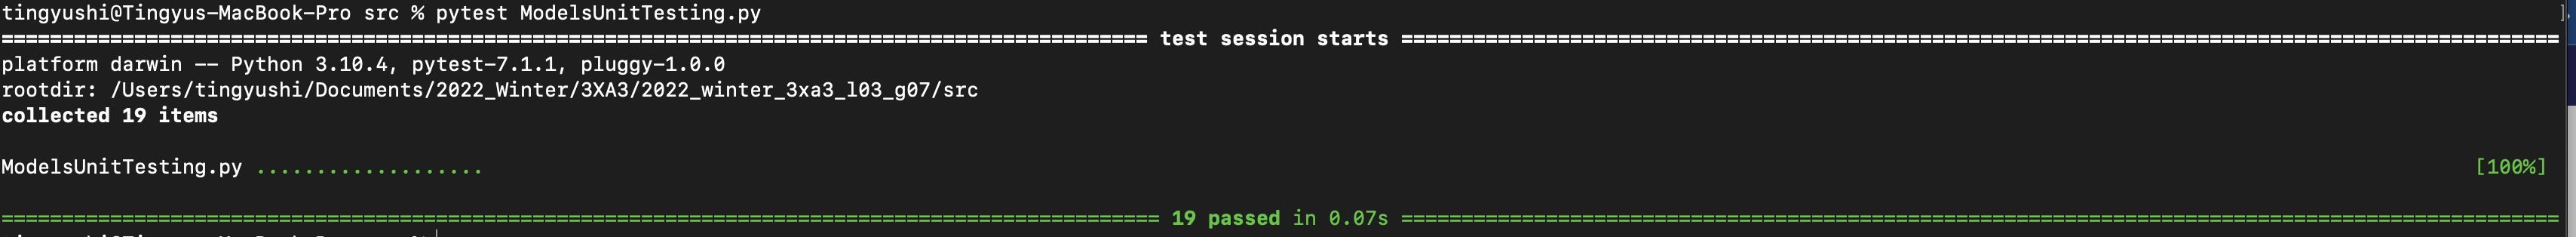
\includegraphics[scale=0.3]{TestResult.png}
\end{center}
\section{Changes Due to Testing}
Through the processes of project, we used functional and not functional tests towards our project. We not only used it to spot errors and fix them, but we also used the tests to improve our project as well. There are a lot of changes we made after doing different aspects of tests.
\subsection{Play Testing}
In the processes of our testing, we mostly used Integration testing to play the game as a whole since it's the most efficient way to test a video game. After playing this game, we found the game is a little boring and that's why we added three more game items in the end to put more elements in this game
\subsection{Difficulty Testing}
During the testing, we focused on testing the difficulty of the game. At the very start, the game is too easy since the speed of enermies' was too slow and speed of bullets from aircraft is too fast. After that, we adjust the speed of bullets of aircraft and monsters to make the game more challenging to play.
\subsection{Music Testing}
The original project has music with it. However, during our play tests, we found that the music is too distracting and annoyinng, so we decided to remove the music from it.
\section{Automated Testing}
Since our project is a game, it requires input from testers all the time. Most of 
our testing is manual testing. However, we used automated testing on our 
game models.
\section{Trace to Requirements}
\begin{table}[htp]
\centering
\caption{Model Traceability Matrix 1}
\begin{tabular}{|c|c|c|c|c|c|c|}
\hline
Tests/Requirement & FR15 & FR16 & FR25 & FR26 & FR27 & FR29 \\
\hline
Test-FR15-M1      & X    &      &      &      &      &      \\
\hline
Test-FR16-M2      &      & X    &      &      &      &      \\
\hline
Test-FR16-M3      &      & X    &      &      &      &      \\
\hline
Test-FR25-M4      &      &      & X    &      &      &      \\
\hline
Test-FR26-M5      &      &      &      & X    &      &      \\
\hline
Test-FR27-M6      &      &      &      &      & X    &      \\
\hline
Test-FR29-M7      &      &      &      &      &      & X\\
\hline   
\end{tabular}
\end{table}

\begin{table}[htp]
\centering
\caption{Model Traceability Matrix 2}
\begin{tabular}{|c|c|c|c|c|c|c|l|}
\hline
Tests/Requirement & FR30 & FR31 & FR32 & FR33 & FR34 & FR35 & FR40 \\
\hline
Test-FR30-M8      & X    &      &      &      &      &        &      \\
\hline
Test-FR31-M9      &      & X    &      &      &      &        &      \\
\hline
Test-FR32-M10     &      &      & X    &      &      &        &      \\
\hline
Test-FR33-M11     &      &      &      & X    &      &        &      \\
\hline
Test-FR34-M12     &      &      &      &      & X    &        &      \\
\hline
Test-FR35-M13   &      &      &      &      &      & X      &      \\
\hline
Test-FR40-M14     &      &      &      &      &      &        & X   \\
\hline
\end{tabular}
\end{table}



\newpage
\subsection{View Traceability Matrices}
\begin{table}[htp]
\centering
\caption{View Traceability Matrix 1}
\begin{tabular}{|c|c|c|c|c|c|c|c|c|c|}
\hline
Tests/Requirement & FR1 & FR2 & FR3 & FR4 & FR5 & FR6 & FR7 & FR8 & FR9 \\
\hline
Test-FR1-V1       & X   &     &     &     &     &     &     &     &     \\
\hline
Test-FR2-V2       &     & X   &     &     &     &     &     &     &     \\
\hline
Test-FR3-V3       &     &     & X   &     &     &     &     &     &     \\
\hline
Test-FR4-V4       &     &     &     & X   &     &     &     &     &     \\
\hline
Test-FR5-V5       &     &     &     &     & X   &     &     &     &     \\
\hline
Test-FR6-V6       &     &     &     &     &     & X   &     &     &     \\
\hline
Test-FR7-V7       &     &     &     &     &     &     & X   &     &     \\
\hline
Test-FR8-V8       &     &     &     &     &     &     &     & X   &     \\
\hline
\end{tabular}
\end{table}
\begin{table}[htp]
\centering
\caption{View Traceability Matrix 2}
\begin{tabular}{|c|c|c|c|c|c|c|c|}
\hline
TestCase\textbackslash{}Requirements & FR9 & FR10 & FR11 & FR12 & FR13 & \textcolor{red}{\st{FR14}}   & FR28 \\ \hline
Test-FR9-V9                          & X   &      &      &      &      &      &      \\ \hline
Test-FR9-V10                         & X   &      &      &      &      &      &      \\ \hline
Test-FR10-V11                        &     & X    &      &      &      &      &      \\ \hline
Test-FR11-V12                        &     &      & X    &      &      &      &      \\ \hline
Test-FR12-V13                        &     &      &      & X    &      &      &      \\ \hline
Test-FR13-V14                        &     &      &      &      & X    &      &      \\ \hline
\textcolor{red}{\st{Test-FR14-V15}}                        &     &      &      &      &      & \textcolor{red}{\st{X}}     &      \\ \hline
Test-FR28-V16                        &     &      &      &      &      &      & X    \\ \hline
Test-FR28-V17                        &     &      &      &      &      &      & X    \\ \hline
Test-FR28-V18                        &     &      &      &      &      &      & X    \\ \hline
\end{tabular}
\end{table}
\newpage
\subsection{Control Traceability Matrices}
\begin{table}[htp]
\centering
\caption{Control Traceability Matrix 1}
\begin{tabular}{|c|c|c|c|c|c|c|}
\hline
Tests/Requirement & FR17 & FR18 & FR19 & FR20 & FR21 & FR22 \\
\hline
Test-FR17-C1      & X    &      &      &      &      &      \\
\hline
Test-FR18-C2      &      & X    &      &      &      &      \\
\hline
Test-FR19-C3      &      &      & X    &      &      &      \\
\hline
Test-FR20-C4      &      &      &      & X    &      &      \\
\hline
Test-FR21-C5      &      &      &      &      & X    &      \\
\hline
Test-FR22-C6      &      &      &      &      &      & X   \\
\hline
\end{tabular}
\end{table}
\noindent \textcolor{red}{For the above table, please only focus on Test-FR18-C2. Other test
cases will not be considered after the revision.}
\begin{table}[htp]
\centering
\caption{Control Traceability Matrix 2}
\begin{tabular}{|c|c|c|c|c|c|c|}
\hline
Tests/Requirement & FR23 & FR24 & FR36 & FR37 & FR38 & \textcolor{red}{\st{FR38}} \\
\hline
Test-FR23-C7      & X    &      &        &      &      &      \\
\hline
Test-FR24-C8      &      & X    &        &      &      &      \\
\hline
Test-FR36-C9    &      &      & X      &      &      &      \\
\hline
Test-FR37-C10     &      &      &        & X    &      &      \\
\hline
Test-FR38-C11     &      &      &        &      & X    &      \\
\hline
\textcolor{red}{\st{Test-FR38-C12}}     &      &      &        &      &      & \textcolor{red}{\st{X}}   \\
\hline
\end{tabular}
\end{table}
\newpage
\subsection{Nonfunctional Req Test Matrices}
\begin{table}[htp]
\centering
\caption{Nonfunctional Req Test Matrix 1}
\begin{tabular}{|c|c|c|c|c|c|c|c|}
\hline
Tests/Requirement & NFR1 & NFR2 & NFR3 & NFR4 & NFR5 & NFR6 & NFR7 \\
\hline
Test-NFR1-LF1     & X    &      &      &      &      &      &      \\
\hline
Test-NFR2-LF2     &      & X    &      &      &      &      &      \\
\hline
Test-NFR3-LF3     &      &      & X    &      &      &      &      \\
\hline
Test-NFR4-LF4     &      &      &      & X    &      &      &      \\
\hline
Test-NFR5-UH1     &      &      &      &      & X    &      &      \\
\hline
Test-NFR6-UH2     &      &      &      &      &      & X    &      \\
\hline
Test-NFR7-UH3     &      &      &      &      &      &      & X\\
\hline   
\end{tabular}
\end{table}
\begin{table}[htp]
\centering
\caption{Nonfunctional Req Test Matrix 2}
\begin{tabular}{|c|c|c|c|c|c|c|c|c|c|}
\hline
Tests/Requirement & NFR8 & NFR9 & NFR10 & NFR11 & NFR12 & NFR13 & \textcolor{red}{\st{NFR14}} & NFR15 & NFR16 \\
\hline
Test-NFR8/9-PE1   & X    & X    &       &       &       &       &       &       &       \\
\hline
Test-NFR10-PE2    &      &      & X     &       &       &       &       &       &       \\
\hline
Test-NFR11-PE3    &      &      &       & X     &       &       &       &       &       \\
\hline
Test-NFR12/13-OE1 &      &      &       &       & X     & X     &       &       &       \\
\hline
\textcolor{red}{\st{Test-NFR14-OE2}}    &      &      &       &       &       &       & \textcolor{red}{\st{X}}     &       &       \\
\hline
Test-NFR15-OE3    &      &      &       &       &       &       &       & X     &       \\
\hline
Test-NFR16-MS1    &      &      &       &       &       &       &       &       & X    \\ \hline
\end{tabular}
\end{table}
\begin{table}[htp]
\centering
\caption{Nonfunctional Req Test Matrix 3}
\begin{tabular}{|c|c|c|c|c|c|c|c|c|}
\hline
Tests/Requirement & NFR17 & NFR18 & NFR19 & NFR20 & \textcolor{red}{\st{NFR21}}  & NFR22 & NFR23 & \textcolor{red}{\st{NFR24}}\\  \hline
Test-NFR17-MS2    & X     &       &       &       &       &       &       &       \\  \hline
Test-NFR18-MS3    &       & X     &       &       &       &       &       &       \\  \hline
Test-NFR19-MS4    &       &       & X     &       &       &       &       &       \\  \hline
Test-NFR20-SE1    &       &       &       & X     &       &       &       &       \\  \hline
\textcolor{red}{\st{Test-NFR21-SE2}}    &       &       &       &       &\textcolor{red}{\st{X}}     &       &       &       \\  \hline
Test-NFR22-CP1    &       &       &       &       &       & X     &       &       \\  \hline
Test-NFR23-LE1    &       &       &       &       &       &       & X     &       \\ \hline
\textcolor{red}{\st{Test-NFR24-HS1}}    &       &       &       &       &       &       &       & \textcolor{red}{\st{X}}    \\ \hline
\end{tabular}
\end{table}
\newpage

\section{Trace to Modules}		
\begin{table}[h!]
\caption{Trace to Modules Table}
\center
\begin{tabular}{|c|c|}
\hline
Test number & Module \\
\hline
Test1 & M1, M2, M17, M14, M18 \\
\hline
Test2 & M17, M15, M1, M2 \\
\hline
Test3 & M1, M2, M23, M15, M17 \\
\hline
Test4 & M14 \\
\hline
Test5 & M14 \\
\hline
Test6 & M14 \\
\hline
Test7 & M17, M31, M19, M1, M2 \\
\hline
Test8 & M6 \\
\hline
Test9 & M16 \\
\hline
Test10 & M24, M1, M2, M16, M14 \\
\hline
Test11 & M22, M15, M1, M2, M17 \\
\hline
Test12 & M23, M15, M1, M2 \\
\hline
Test13 & M16\\
\hline
Test14 & M15, M1, M2 \\
\hline
Test15 & M12, M1 \\
\hline
Test16 & M27, M1 \\
\hline
Test17 & M27, M1 \\
\hline
Test18 & M8 \\
\hline
Test19 & M10 \\
\hline
Test20 & M13 \\
\hline
Test21 & M6 \\
\hline
Test22 & M6, M14 \\
\hline
Test23 & M5, M3 \\
\hline
Test24 & M5, M3 \\
\hline
Test25 & M9 \\
\hline
Test26 & M8\\
\hline
Test27 & M3, M30 \\
\hline
Test28 & M29, M3 \\
\hline
Test29 & M6, M1, M2 \\
\hline
Test30 & M6, M1, M2 \\
\hline
Test31 & M6, M1, M2 \\
\hline
Test32 & M1, M2, M16 \\
\hline
Test33 & M6, M16 \\
\hline
Test34 & M16 \\
\hline
Test35 & M3 \\
\hline
Test36 & M3 \\
\hline
Test37 & M15\\
\hline
\end{tabular}
\end{table}
\noindent The reason why we only include functional requirements here is because for the non-functional requirements, it's not applicable to trace them to specific modules since some of them are tested by interviews and tested subjectively.


\section{Code Coverage Metrics}
The code coverage of this project is only 33 percent because at most of the time we use integration test to test the whole game. For controller and view modules, most of the lines cannot be reached since they depend on certain input from the user. The 
following is the screenshot of our code coverage:
\begin{center}
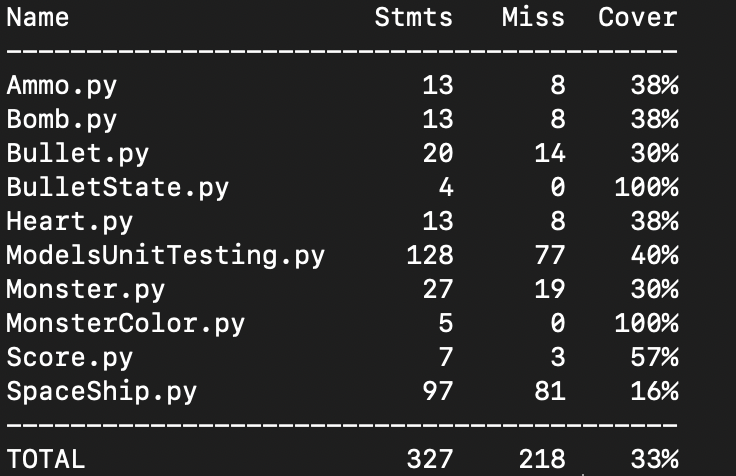
\includegraphics[scale=1]{CodeCoverage.png}
\end{center}
\bibliographystyle{plainnat}


\end{document}